\section{Módulo de Almacenamiento de Datos}
\label{sec:decentralized_tech_traffic_storage}

El módulo \texttt{traffic-storage} actúa como capa de persistencia verificable del sistema, recibiendo métricas de tráfico y resultados de optimización, almacenando los datos en un repositorio distribuido y registrando huellas inmutables en infraestructuras descentralizadas. En este contexto, blockchain, BlockDAG e IPFS se utilizan de forma complementaria: blockchain y BlockDAG como ledgers inmutables para trazabilidad, e IPFS como almacén de archivos orientado a contenido \cite{nakamoto2008bitcoin,benet2014ipfs,sompolinsky2021phantom}.

% -----------------------------------------------------------------------------
\subsection{Blockchain}
\label{subsec:blockchain_traffic_storage}

Blockchain puede describirse como un libro mayor distribuido donde las transacciones se agrupan en bloques enlazados criptográficamente en una cadena lineal, de modo que cada bloque referencia al anterior mediante un resumen criptográfico (hash), proporcionando inmutabilidad y resistencia a manipulaciones retrospectivas \cite{nakamoto2008bitcoin,narayanan2016bitcoin}. Los nodos de la red ejecutan un mecanismo de consenso (como Proof-of-Work o Proof-of-Stake) para acordar qué bloques se consideran válidos, garantizando que todos mantengan una vista consistente del historial de transacciones \cite{buterin2014ethereum,garay2015backbone}.

La Figura~\ref{fig:bloque_blockchain} ilustra la estructura básica de una cadena de bloques, mostrando cómo cada bloque referencia criptográficamente al bloque anterior mediante su resumen criptográfico (hash), creando una cadena inmutable donde cualquier modificación en un bloque anterior invalida todos los bloques subsiguientes.

\begin{figure}[htbp]
    \centering
    \shorthandoff{>}
    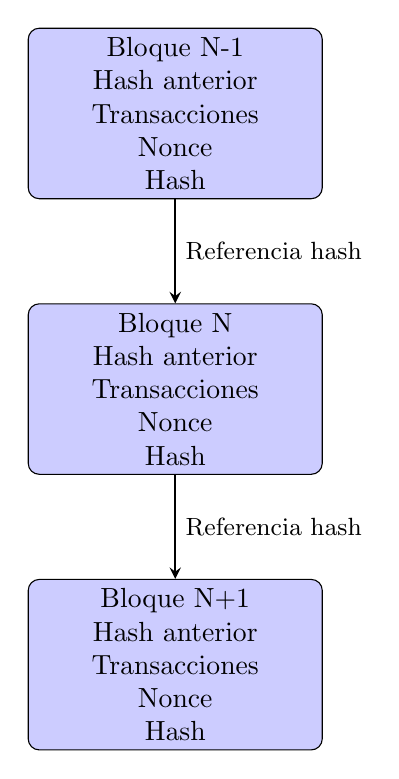
\begin{tikzpicture}[
        block/.style={rectangle, draw, fill=blue!20,
                      text width=3.5cm, text centered,
                      rounded corners, minimum height=2cm},
        arrow/.style={->,thick,>=stealth}
    ]
    
        % Bloques más separados verticalmente
        \node[block] (bloque1) at (0,7) {Bloque N-1 \\ Hash anterior \\ Transacciones \\ Nonce \\ Hash};
        \node[block] (bloque2) at (0,3.5) {Bloque N \\ Hash anterior \\ Transacciones \\ Nonce \\ Hash};
        \node[block] (bloque3) at (0,0) {Bloque N+1 \\ Hash anterior \\ Transacciones \\ Nonce \\ Hash};
    
        % Flechas largas con etiqueta pegada
        \draw[arrow] (bloque1.south) -- node[midway,right]{\small Referencia hash} (bloque2.north);
        \draw[arrow] (bloque2.south) -- node[midway,right]{\small Referencia hash} (bloque3.north);
    
    \end{tikzpicture}
    \shorthandon{>}
    \caption{Estructura básica de una cadena de bloques, mostrando la dependencia criptográfica entre bloques consecutivos \cite{nakamoto2008bitcoin}.}
    \label{fig:bloque_blockchain}
\end{figure}

En este trabajo, blockchain se utiliza para registrar metadatos de almacenamiento de tráfico de forma inmutable, actuando como capa de ``prueba de existencia'' para datos que residen físicamente fuera de la cadena. El contrato inteligente de almacenamiento expone operaciones de alto nivel para registrar eventos de almacenamiento: cada llamada almacena, al menos, un identificador de semáforo, una marca de tiempo y un identificador de contenido (CID de IPFS), junto con el tipo de dato al que hace referencia. Este contrato se despliega y prueba utilizando un entorno de desarrollo estándar, con scripts de despliegue y pruebas automatizadas que verifican su funcionamiento básico.

El módulo \texttt{traffic-storage} ofrece una API HTTP que recibe cargas de datos en un formato unificado (versión 2.0), generadas por otros componentes del sistema (como los módulos de optimización y lógica difusa). Cuando llega una nueva medición o reporte, la API valida la carga útil, delega la persistencia de contenido a IPFS y, una vez obtenido el CID, invoca al contrato inteligente de almacenamiento para registrar ese CID junto con los metadatos relevantes en la blockchain. De este modo, los algoritmos de optimización y los módulos de monitoreo solo interactúan con una interfaz REST, mientras que los detalles de interacción on-chain quedan encapsulados en el módulo de almacenamiento.

% -----------------------------------------------------------------------------
\subsection{BlockDAG}
\label{subsec:blockdag_traffic_storage}

BlockDAG (Block Directed Acyclic Graph) generaliza la estructura lineal de blockchain permitiendo que cada bloque referencie a múltiples bloques padres anteriores, formando un grafo dirigido acíclico en lugar de una cadena única \cite{wang2023dag,sompolinsky2021phantom}. Esta arquitectura permite que bloques creados en paralelo se integren en el consenso sin ser descartados como huérfanos, mejorando el aprovechamiento del ancho de banda de la red y posibilitando mayores tasas de transacciones y menores latencias de confirmación que las típicamente alcanzables en cadenas lineales \cite{wang2023dag}.

La Tabla~\ref{tab:blockchain_vs_blockdag} sintetiza las principales diferencias entre arquitecturas blockchain tradicionales y BlockDAG basadas en protocolos como GHOSTDAG. La comparación considera protocolos representativos de cada paradigma: Nakamoto consensus implementado en Bitcoin y Ethereum para blockchains lineales \cite{nakamoto2008bitcoin,buterin2014ethereum}, y PHANTOM/GHOSTDAG como generalización del consenso distribuido en estructuras DAG \cite{sompolinsky2021phantom}.

\begin{table}[htbp]
\renewcommand{\arraystretch}{1.3}
\caption{Comparación entre Blockchain Tradicional y BlockDAG}
\label{tab:blockchain_vs_blockdag}
\centering
\footnotesize
\begin{tabular}{lcc}
\hline
\textbf{Característica} & \textbf{Blockchain Tradicional} & \textbf{BlockDAG (GHOSTDAG)} \\
\hline
Topología & Lineal (1 padre)\cite{sompolinsky2021phantom} & Grafo acíclico (múltiples padres)\cite{sompolinsky2021phantom,zhang2025sok} \\
Bloques huérfanos & Descartados\cite{sompolinsky2021phantom} & Integrados como padres\cite{sompolinsky2021phantom} \\
Ordenamiento & Total (intrínseco) & Parcial $\rightarrow$ Total (vía algoritmo)\cite{sompolinsky2021phantom} \\
Escalabilidad & Limitada\cite{sompolinsky2021phantom} & Alta (ancho de banda físico)\cite{sompolinsky2021phantom,zhang2025sok} \\
Confirmación & Probabilística lenta & Probabilística rápida (segundos)\cite{zhang2025sok} \\
Minería & Competitiva\cite{sompolinsky2021phantom} & Cooperativa\cite{sompolinsky2021phantom} \\
Throughput típico & 7-30 TPS\cite{nakamoto2008bitcoin,buterin2014ethereum} & 100+ TPS\cite{zhang2025sok} \\
Latencia de bloque & 10 min (Bitcoin), 12 s (Ethereum)\cite{ethereum_blocks} & Sub-segundo a segundos\cite{zhang2025sok} \\
\hline
\end{tabular}
\end{table}

En el contexto de este sistema, BlockDAG se considera como infraestructura de registro distribuido complementaria a la blockchain tradicional, pensada para escenarios de mayor escala donde múltiples intersecciones reportan datos con alta frecuencia. El módulo \texttt{traffic-storage} incorpora una capa de abstracción que permite, según la configuración, registrar eventos de almacenamiento tanto en un contrato EVM como en una red BlockDAG compatible, utilizando un cliente dedicado que construye y envía mensajes de registro a un nodo remoto. Estos mensajes contienen, de forma análoga a la variante blockchain, el identificador de semáforo, la marca de tiempo y el resumen criptográfico de contenido (CID de IPFS u otro identificador criptográfico).

La lógica de alto nivel en el módulo de almacenamiento se mantiene independiente de la tecnología subyacente: la API recibe métricas y resultados de optimización, delega la persistencia de archivos a IPFS y, posteriormente, invoca una interfaz de "registro de evidencia" que puede mapearse a blockchain, BlockDAG o a un esquema dual. Esta separación permite que, a medida que se exploren o adopten redes DAG de mayor throughput para despliegues reales en entornos de ciudad inteligente, el resto del sistema (clasificación de congestión, PSO, paneles de monitoreo) continúe interactuando con un mismo punto de entrada consistente.

% -----------------------------------------------------------------------------
\subsection{IPFS}
\label{subsec:ipfs_traffic_storage}

El InterPlanetary File System (IPFS) es un sistema de archivos distribuido peer-to-peer que utiliza direccionamiento por contenido: cada objeto se identifica por un Content Identifier (CID) que codifica un resumen criptográfico (hash) del contenido más metadatos mínimos sobre cómo interpretarlo \cite{benet2014ipfs}. El mismo archivo siempre produce el mismo CID, independientemente del nodo que lo procese, lo que permite verificar integridad de manera determinista y realizar deduplicación automática a escala de red \cite{ipfs_architecture}.

La Figura~\ref{fig:ipfs_architecture} ilustra el flujo básico de almacenamiento y recuperación en IPFS, mostrando cómo un archivo se fragmenta, se le asigna un CID basado en su contenido, y puede ser recuperado desde cualquier nodo que posea los bloques correspondientes.

\begin{figure}[htbp]
    \centering
    \shorthandoff{>}
    \begin{tikzpicture}[
        node distance=1.5cm,
        block/.style={rectangle, draw, rounded corners, fill=green!10,
                      text width=3cm, text centered, minimum height=1cm},
        storage/.style={cylinder, draw, shape border rotate=90, aspect=0.25, 
                       fill=blue!10, minimum height=1.2cm, minimum width=2cm},
        arrow/.style={->,thick,>=stealth}
    ]
    
        % Archivo original
        \node[block] (file) {Archivo\\datos.json};
        
        % Fragmentación
        \node[block, below=of file] (fragment) {Fragmentación\\en bloques};
        
        % Bloques
        \node[storage, below left=1.5cm and 0.5cm of fragment] (block1) {Bloque 1};
        \node[storage, below=1.5cm of fragment] (block2) {Bloque 2};
        \node[storage, below right=1.5cm and 0.5cm of fragment] (block3) {Bloque N};
        
        % CID
        \node[block, fill=orange!20, below=3.5cm of fragment] (cid) {CID\\QmX...ABC};
        
        % Red IPFS
        \node[block, fill=purple!10, below=of cid] (network) {Red IPFS\\distribuida};
        
        % Recuperación
        \node[block, right=4cm of network] (retrieve) {Recuperación\\mediante CID};
        
        % Flechas
        \draw[arrow] (file) -- (fragment);
        \draw[arrow] (fragment) -- (block1);
        \draw[arrow] (fragment) -- (block2);
        \draw[arrow] (fragment) -- (block3);
        \draw[arrow] (block1) -- (cid);
        \draw[arrow] (block2) -- (cid);
        \draw[arrow] (block3) -- (cid);
        \draw[arrow] (cid) -- (network);
        \draw[arrow, dashed] (network) -- node[above]{\small Solicitud} (retrieve);
        \draw[arrow, dashed] (retrieve) -- node[below]{\small Bloques} (network);
    
    \end{tikzpicture}
    \shorthandon{>}
    \caption{Arquitectura básica de IPFS: fragmentación de archivos, generación de CID y recuperación distribuida \cite{benet2014ipfs}.}
    \label{fig:ipfs_architecture}
\end{figure}

En este trabajo, IPFS se emplea como almacén de datos off-chain para los artefactos generados y consumidos por el sistema: mediciones agregadas de tráfico por grupo (clúster), indicadores de congestión difusa, configuraciones optimizadas de tiempos semafóricos y reportes experimentales. El módulo \texttt{traffic-storage} incluye un cliente específico para interactuar con un nodo IPFS local o con un servicio compatible, ofreciendo operaciones sencillas para subir y recuperar objetos. El flujo básico consiste en que la API recibe una carga útil de datos, lo serializa (por ejemplo, como JSON), lo envía al nodo IPFS y obtiene de vuelta un CID.

Ese CID se utiliza a continuación como enlace entre IPFS y las capas de consenso: se registra en blockchain o en BlockDAG mediante las interfaces descritas anteriormente, de modo que cualquier módulo que necesite auditar o reanalizar un conjunto de datos solo requiera conocer el CID y el identificador de semáforo asociado. Desde la perspectiva del resto del sistema, IPFS y las tecnologías de registro inmutable quedan encapsuladas detrás del módulo de almacenamiento: los módulos de simulación, clasificación difusa y optimización interactúan únicamente con la API REST, mientras que las garantías de verificabilidad, integridad y persistencia se logran combinando direccionamiento por contenido en IPFS con registros inmutables en blockchain y/o BlockDAG.

La Figura~\ref{fig:storage_sequence} presenta un diagrama de secuencia que ilustra el flujo completo de almacenamiento distribuido: desde la recepción de datos por la API hasta el registro del CID en la capa de consenso, mostrando la interacción entre los componentes del módulo de almacenamiento.

\begin{figure}[htbp]
    \centering
    \shorthandoff{>}
    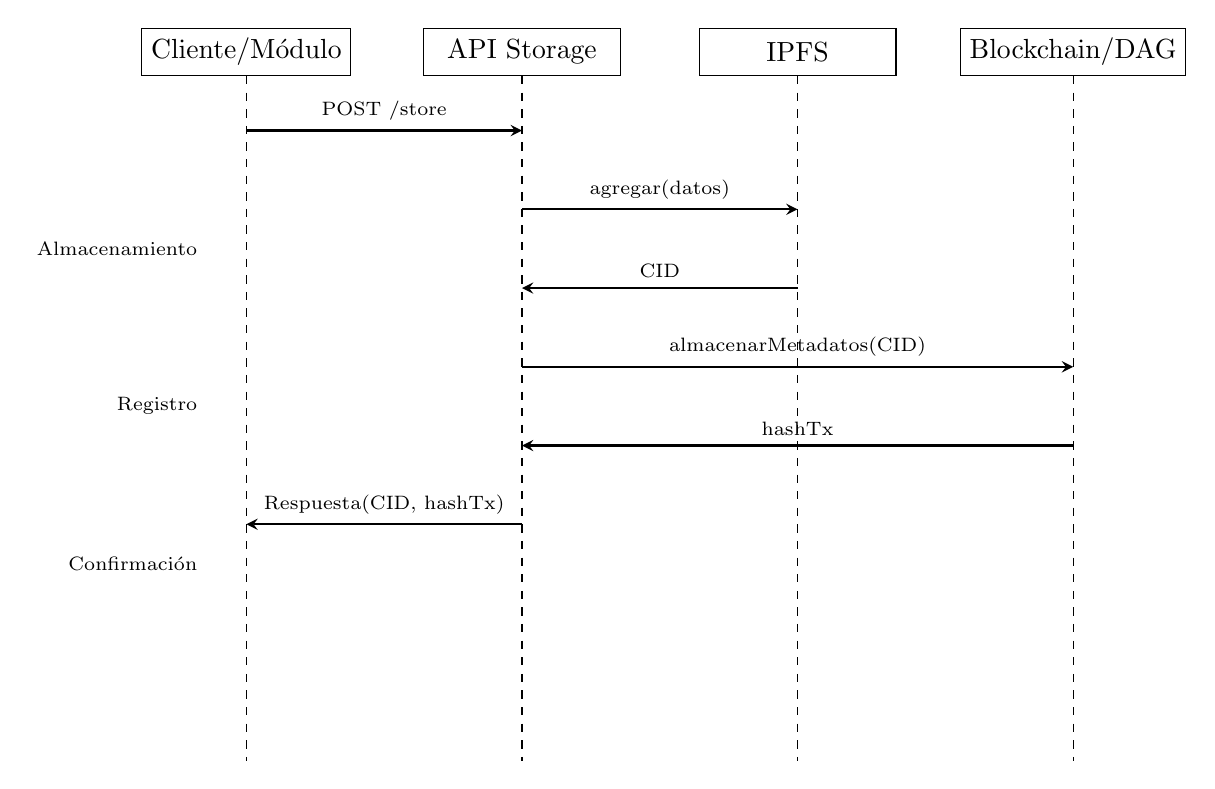
\begin{tikzpicture}[
        >=stealth,
        node distance=0.8cm,
        actor/.style={rectangle, draw, minimum width=2.5cm, minimum height=0.6cm},
        message/.style={->,thick}
    ]
    
        % Actores
        \node[actor] (client) at (0,0) {Cliente/Módulo};
        \node[actor] (api) at (3.5,0) {API Storage};
        \node[actor] (ipfs) at (7,0) {IPFS};
        \node[actor] (blockchain) at (10.5,0) {Blockchain/DAG};
        
        % Líneas de vida
        \draw[dashed] (client) -- ++(0,-9);
        \draw[dashed] (api) -- ++(0,-9);
        \draw[dashed] (ipfs) -- ++(0,-9);
        \draw[dashed] (blockchain) -- ++(0,-9);
        
        % Mensajes
        \draw[message] (0,-1) -- node[above,font=\scriptsize] {POST /store} (3.5,-1);
        
        \draw[message] (3.5,-2) -- node[above,font=\scriptsize] {agregar(datos)} (7,-2);
        \draw[message] (7,-3) -- node[above,font=\scriptsize] {CID} (3.5,-3);
        
        \draw[message] (3.5,-4) -- node[above,font=\scriptsize] {almacenarMetadatos(CID)} (10.5,-4);
        \draw[message] (10.5,-5) -- node[above,font=\scriptsize] {hashTx} (3.5,-5);
        
        \draw[message] (3.5,-6) -- node[above,font=\scriptsize] {Respuesta(CID, hashTx)} (0,-6);
        
        % Etiquetas de secciones
        \node[left] at (-0.5,-2.5) {\scriptsize Almacenamiento};
        \node[left] at (-0.5,-4.5) {\scriptsize Registro};
        \node[left] at (-0.5,-6.5) {\scriptsize Confirmación};
    
    \end{tikzpicture}
    \shorthandon{>}
    \caption{Diagrama de secuencia del flujo de almacenamiento distribuido en \texttt{traffic-storage}.}
    \label{fig:storage_sequence}
\end{figure}

